\section{Results, Demonstration and Discussion}

\subsection{Implemented Features}
\begin{table}[H]
\centering
\caption{Implementation status of features (implemented = code + automated test)}
\label{tab:features}
\small
\begin{tabularx}{\textwidth}{@{}Xp{2.4cm}p{3.3cm}@{}}
\toprule
\textbf{Feature} & \textbf{Status} & \textbf{Evidence}\\
\midrule
Login, activation, password reset, 5 roles with server-side RBAC & Implemented, tested & test\_auth (15)\\
Upload PDF / scanned PDF / image / XLSX / XLS / CSV / DOCX / DOC & Implemented, tested & test\_extraction (24)\\
Extraction tuned on real college PDF (labs, legends, noon row, BE combined, LLC) & Implemented, tested & test\_reference\_pdf (14)\\
Validation, review \& correction (audited), activation, archives & Implemented, tested & test\_uploads (13)\\
Conflict detection (professor / room / batch) & Implemented, tested & 2 genuine clashes found\\
Role dashboards, weekly view, class details & Implemented, e2e tested & Figures \ref{fig:screens1}--\ref{fig:screens2}\\
Natural-language search: compositional query plans (count, first/last, per day, lab/lecture, before/after) plus specialised operations, clarifications & Implemented, tested & test\_query\_engine (59), composed tests (7)\\
Personal timetables, strictly separate & Implemented, tested & domain tests\\
Promotion, fresher registration, master data, users, audit log & Implemented, tested & test\_academics (13)\\
Android, iPhone (Expo Go), laptop browser & Implemented; web e2e; device tried & Screenshots\\
Free online demo (Render) & Deployed & \texttt{render.yaml}, demo link\\
Push notifications & Implemented, not verified & Needs store build\\
E-mail delivery (SMTP) & Implemented, not verified & No mail server configured\\
Installable store apps (APK/TestFlight) & Configured (EAS), not built & --\\
\bottomrule
\end{tabularx}
\end{table}

\subsection{Screenshots and Demonstration Evidence}
The screenshots below were captured automatically by the Playwright end-to-end tests running the real
app (web build, phone-sized viewport) against the real API, with the college's timetable loaded.

\begin{figure}[H]
\centering

\includegraphics[width=0.75\textwidth]{figures/real-pdf-page1.png}
\caption{Input: page 1 of the college's real timetable PDF (S.E.\ Division A), with stacked lab cells and legend}
\label{fig:realpdf}
\end{figure}

\begin{figure}[H]
\centering
\begin{subfigure}[t]{0.24\textwidth}\centering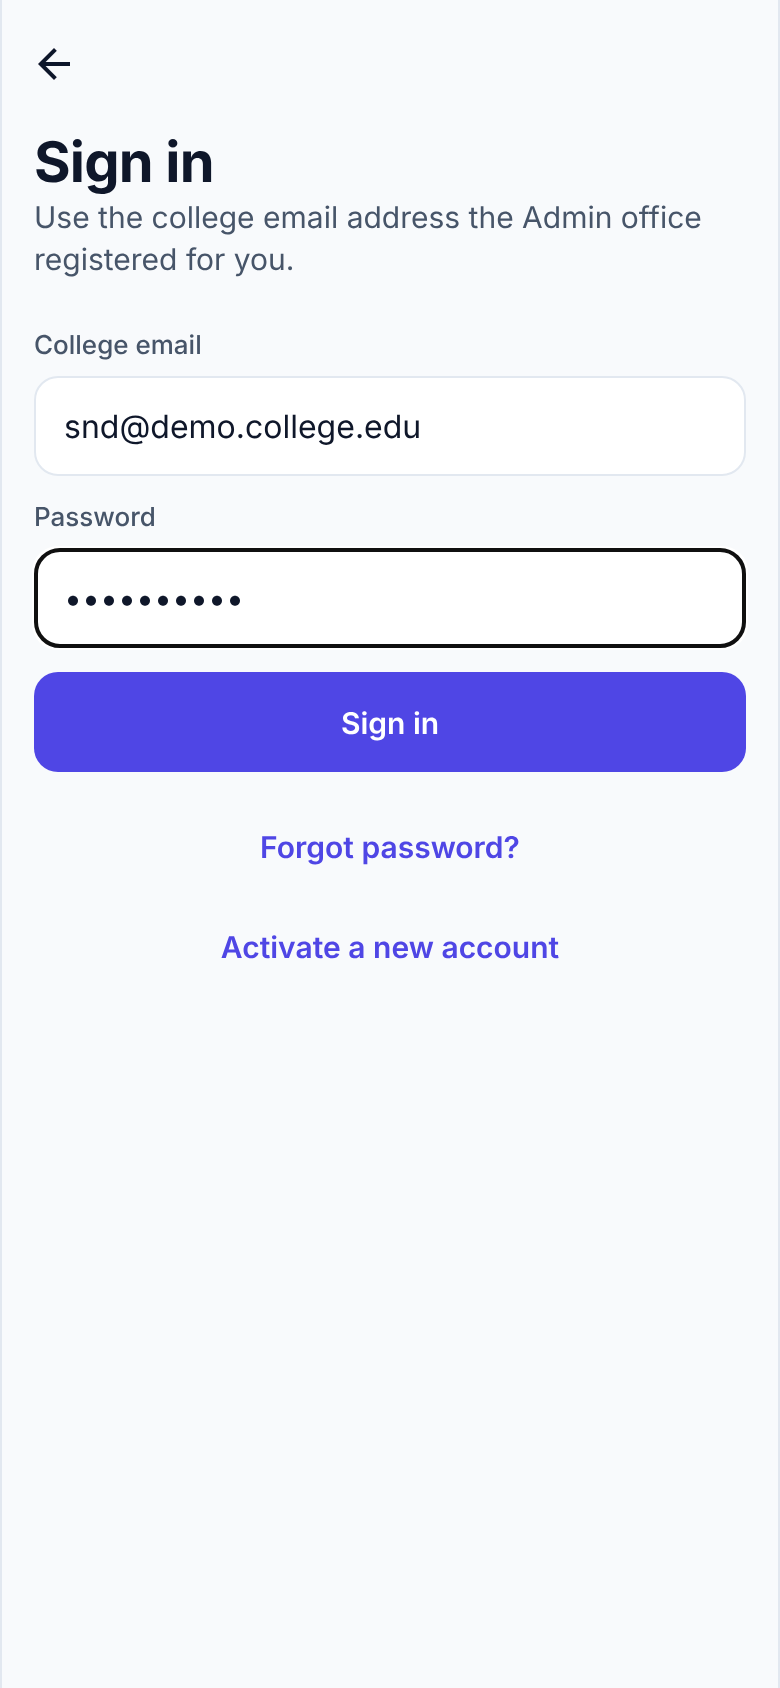
\includegraphics[width=\linewidth]{figures/screens/login.png}\caption{Sign in}\end{subfigure}\hfill
\begin{subfigure}[t]{0.24\textwidth}\centering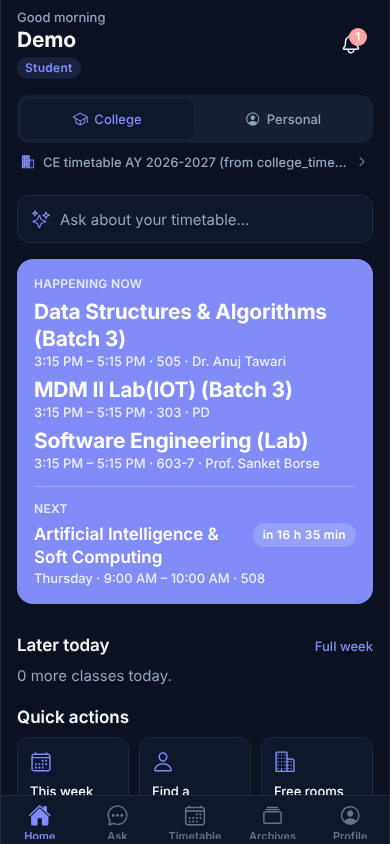
\includegraphics[width=\linewidth]{figures/screens/home-dark.png}\caption{Student home (dark mode): now / next}\end{subfigure}\hfill
\begin{subfigure}[t]{0.24\textwidth}\centering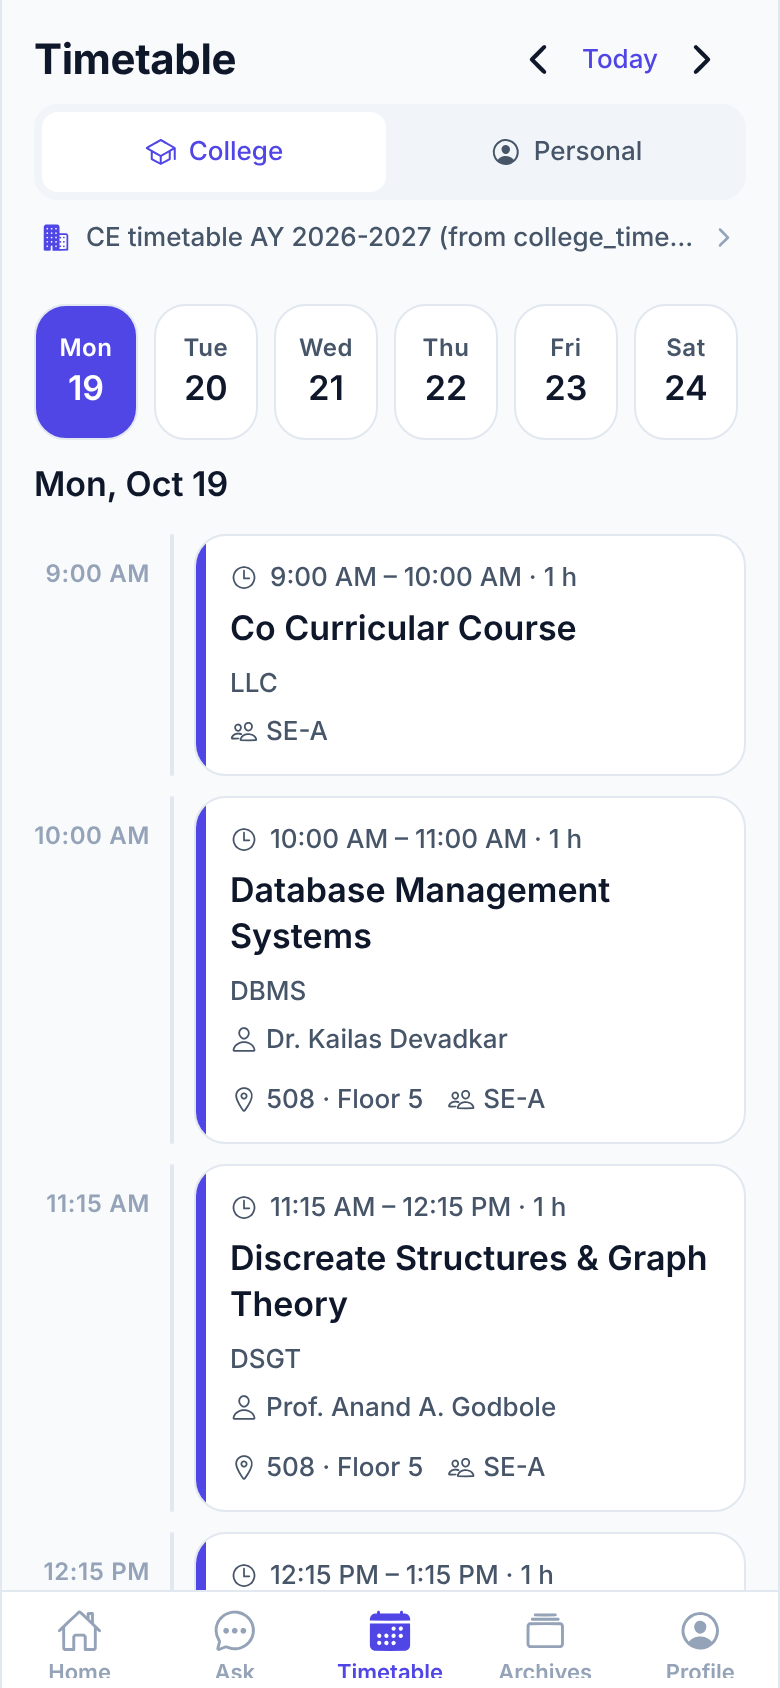
\includegraphics[width=\linewidth]{figures/screens/student-monday.png}\caption{Week view, Monday (SE-A1)}\end{subfigure}\hfill
\begin{subfigure}[t]{0.24\textwidth}\centering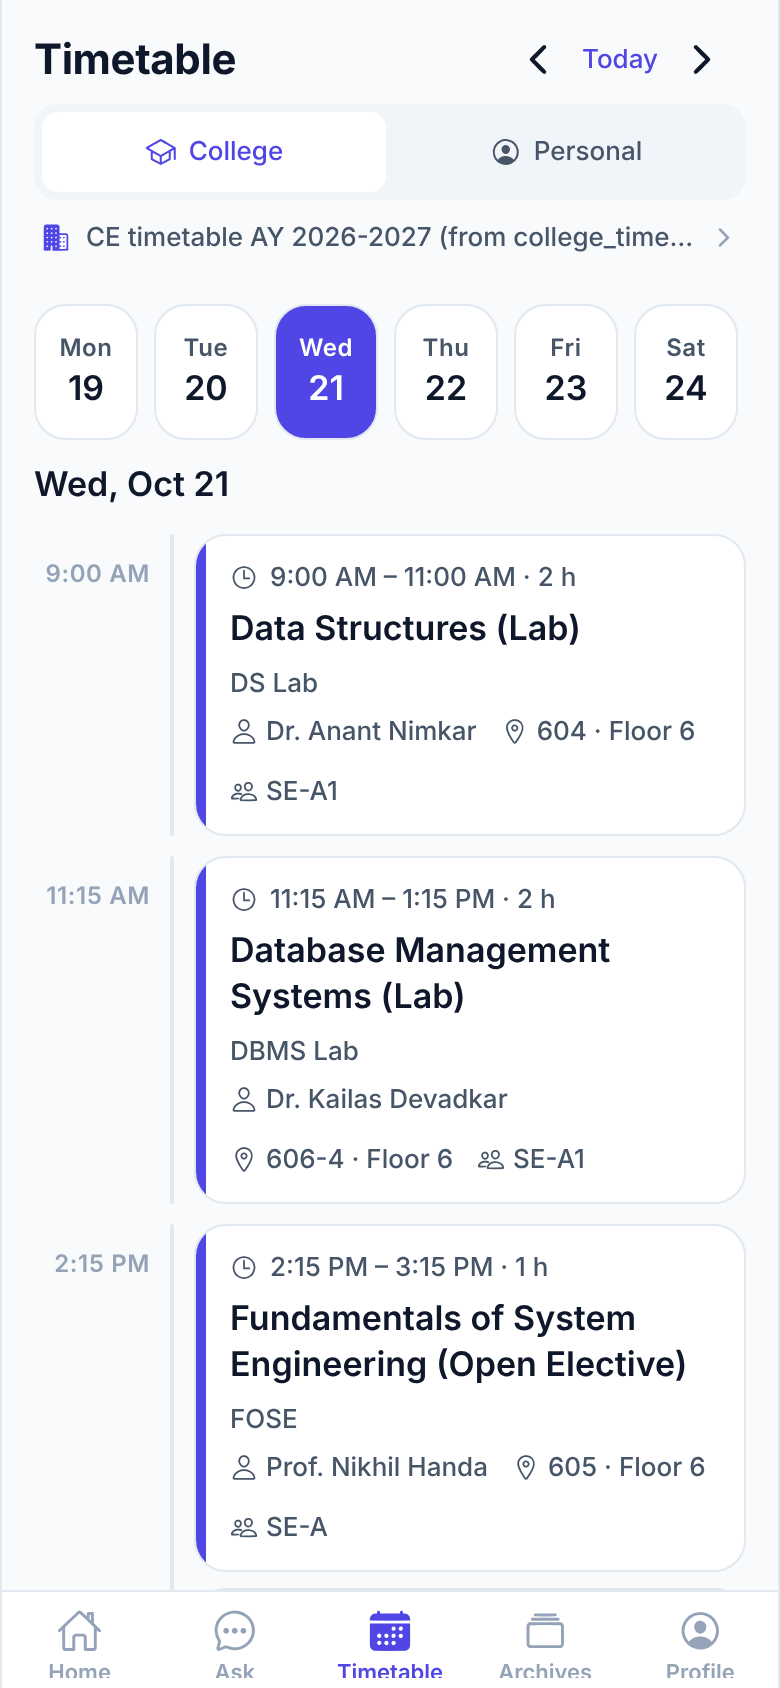
\includegraphics[width=\linewidth]{figures/screens/student-wednesday-lab.png}\caption{Only lab group A1's labs}\end{subfigure}
\caption{Student screens}
\label{fig:screens1}
\end{figure}

\begin{figure}[H]
\centering
\begin{subfigure}[t]{0.24\textwidth}\centering
\includegraphics[width=\linewidth]{figures/screens/class-details.png}\caption{Class details with source page and raw text (LLC: no teacher/room)}\end{subfigure}\hfill
\begin{subfigure}[t]{0.24\textwidth}\centering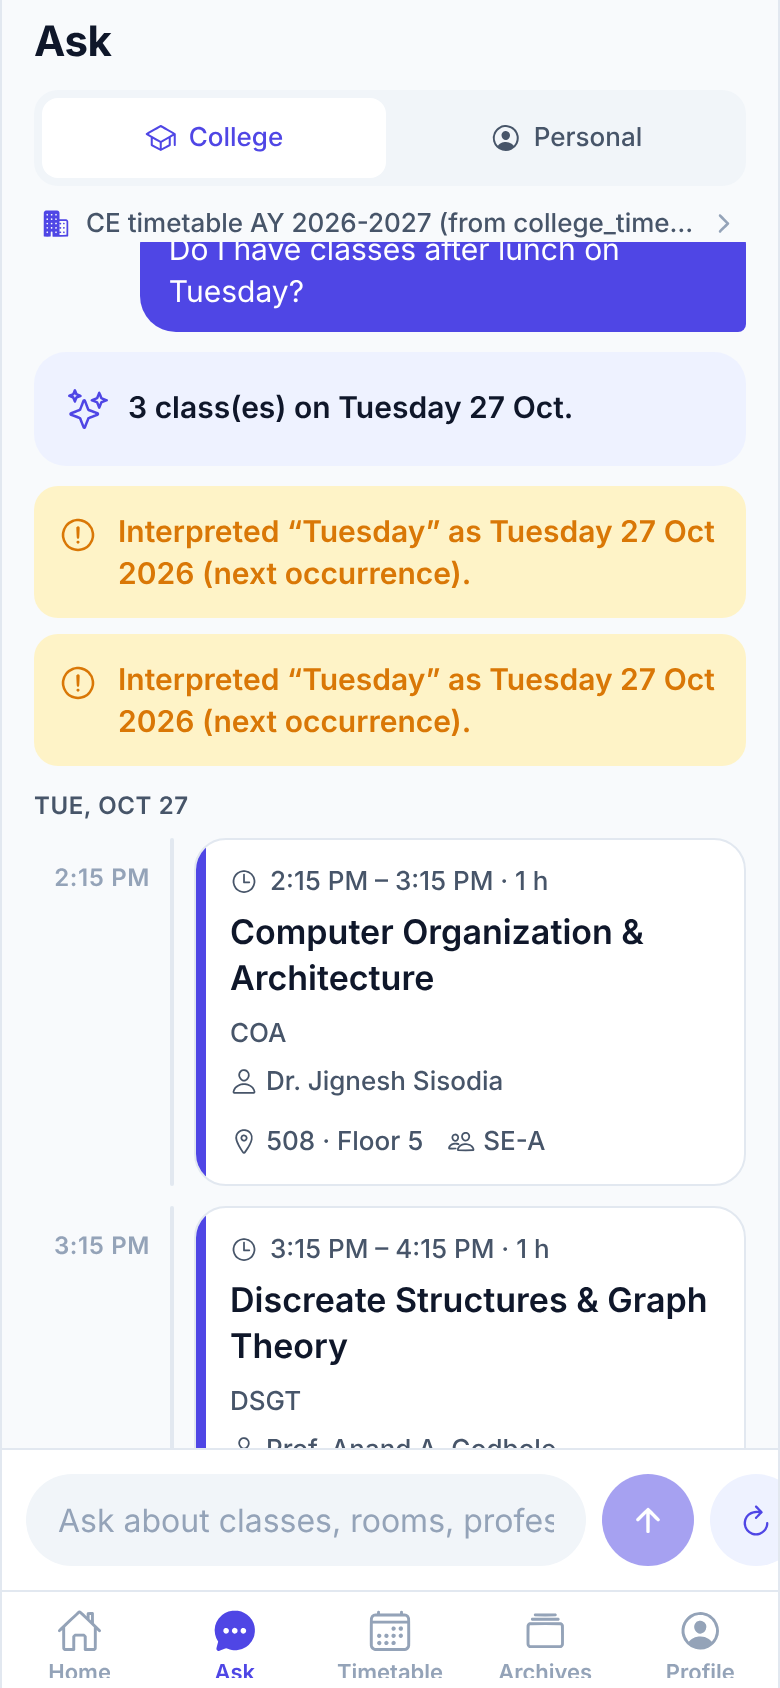
\includegraphics[width=\linewidth]{figures/screens/ask-after-lunch.png}\caption{``Classes after lunch on Tuesday?'' uses SE lunch}\end{subfigure}\hfill
\begin{subfigure}[t]{0.24\textwidth}\centering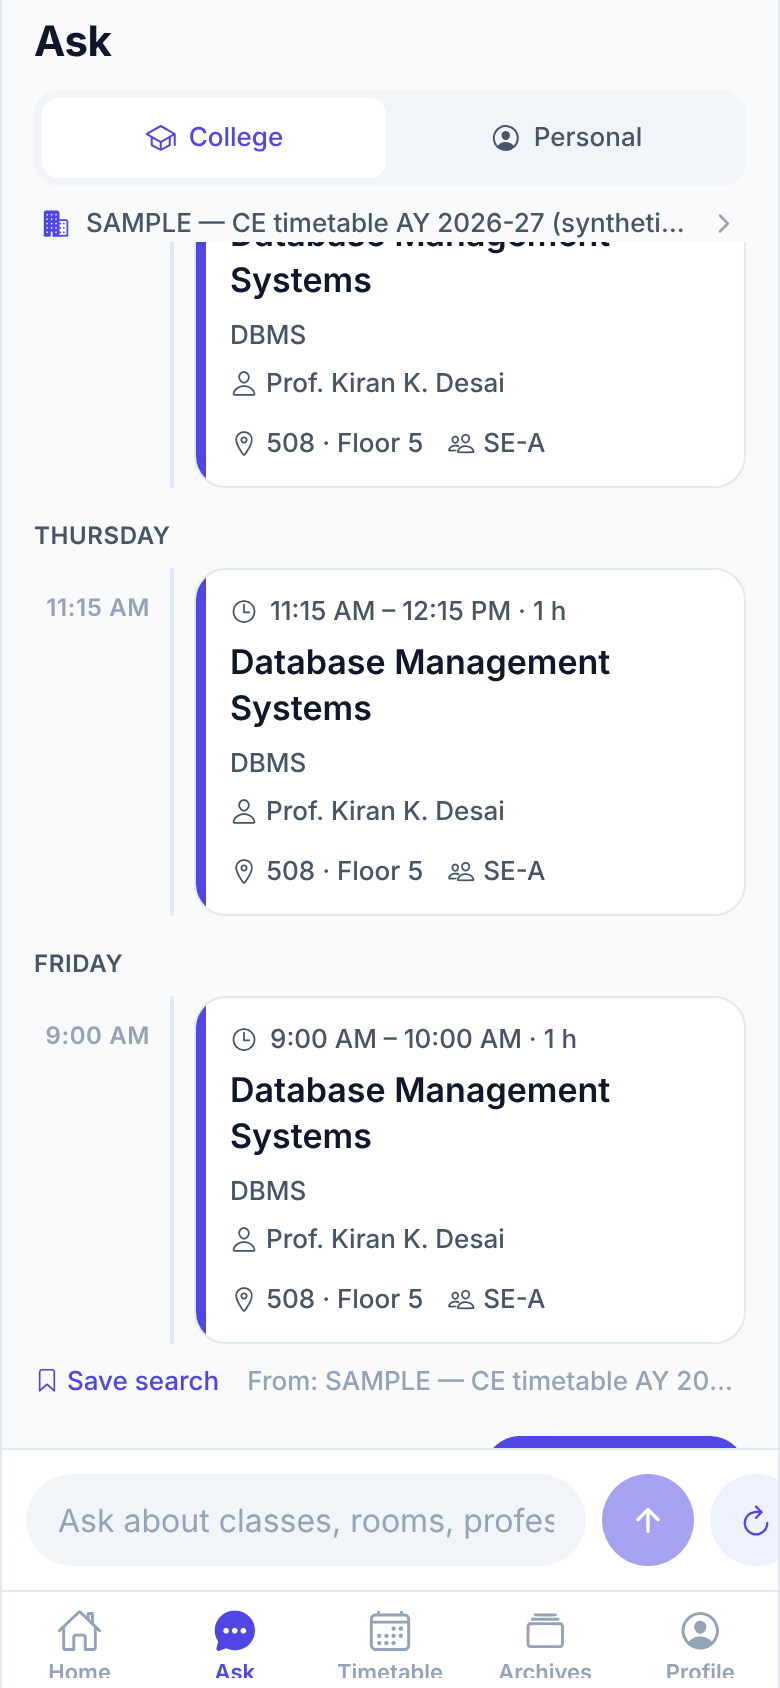
\includegraphics[width=\linewidth]{figures/screens/clarify-ampm.png}\caption{``Am I free at 2?'' asks a.m.\ or p.m.}\end{subfigure}\hfill
\begin{subfigure}[t]{0.24\textwidth}\centering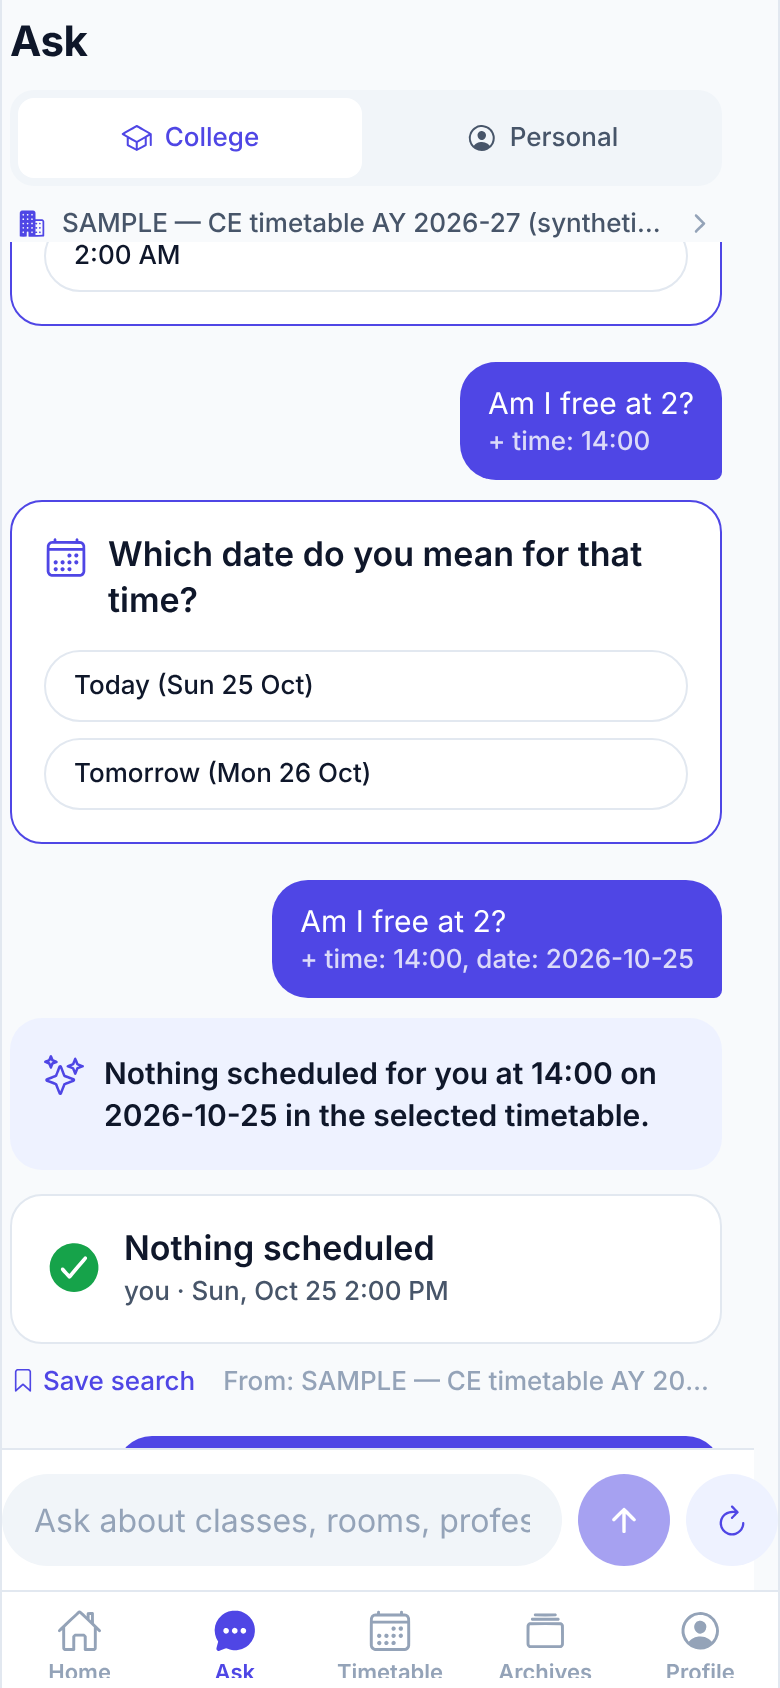
\includegraphics[width=\linewidth]{figures/screens/cross-domain.png}\caption{After choosing 2 PM and the date: answer}\end{subfigure}
\caption{Natural-language search (Ask tab)}
\label{fig:screensask}
\end{figure}

\begin{figure}[H]
\centering
\begin{subfigure}[t]{0.24\textwidth}\centering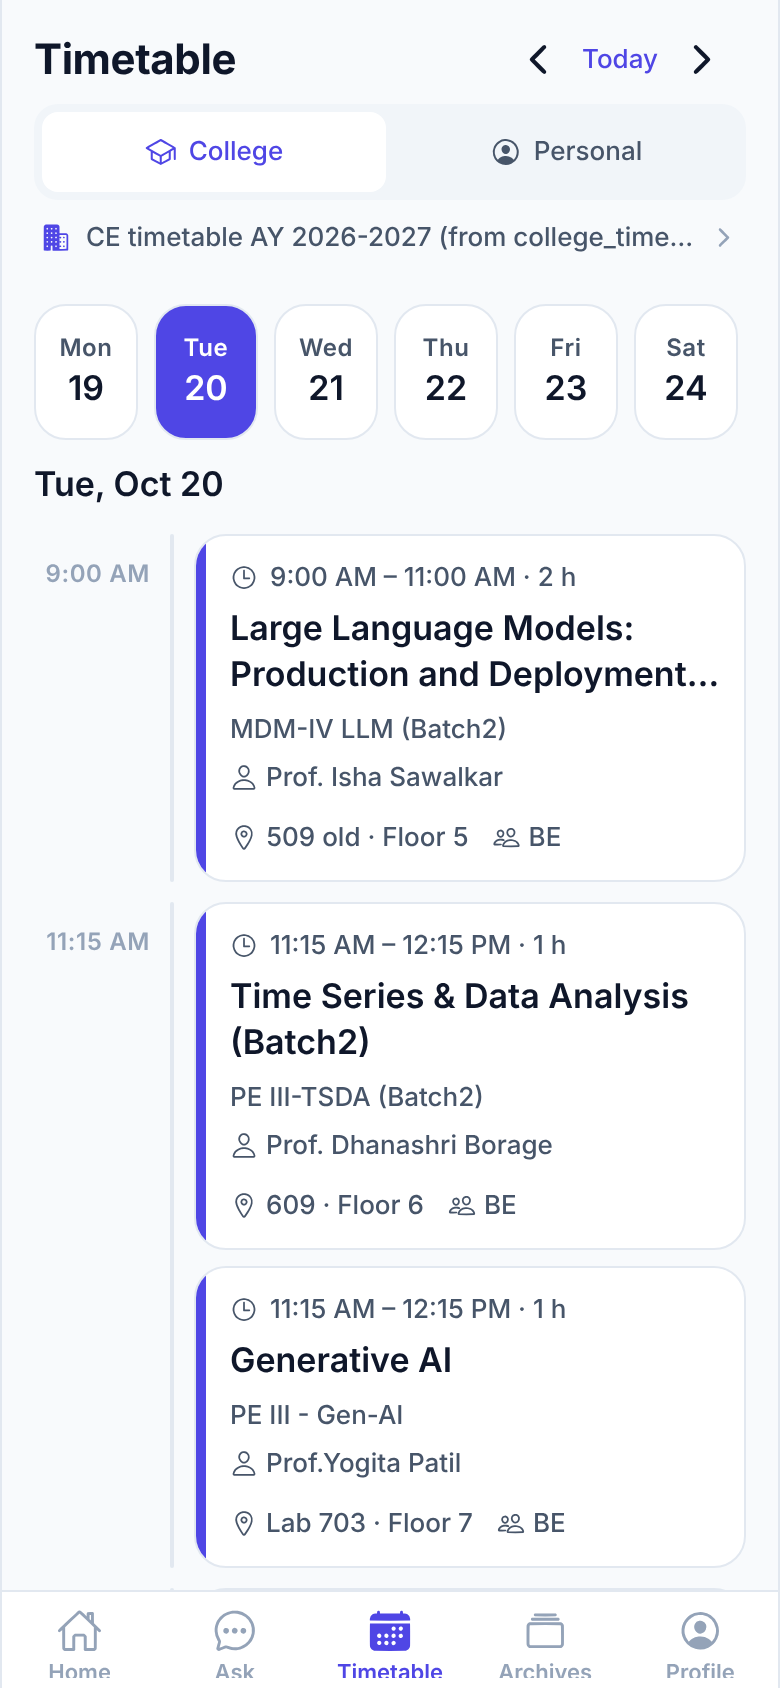
\includegraphics[width=\linewidth]{figures/screens/be-combined.png}\caption{B.E.\ combined electives}\end{subfigure}\hfill
\begin{subfigure}[t]{0.24\textwidth}\centering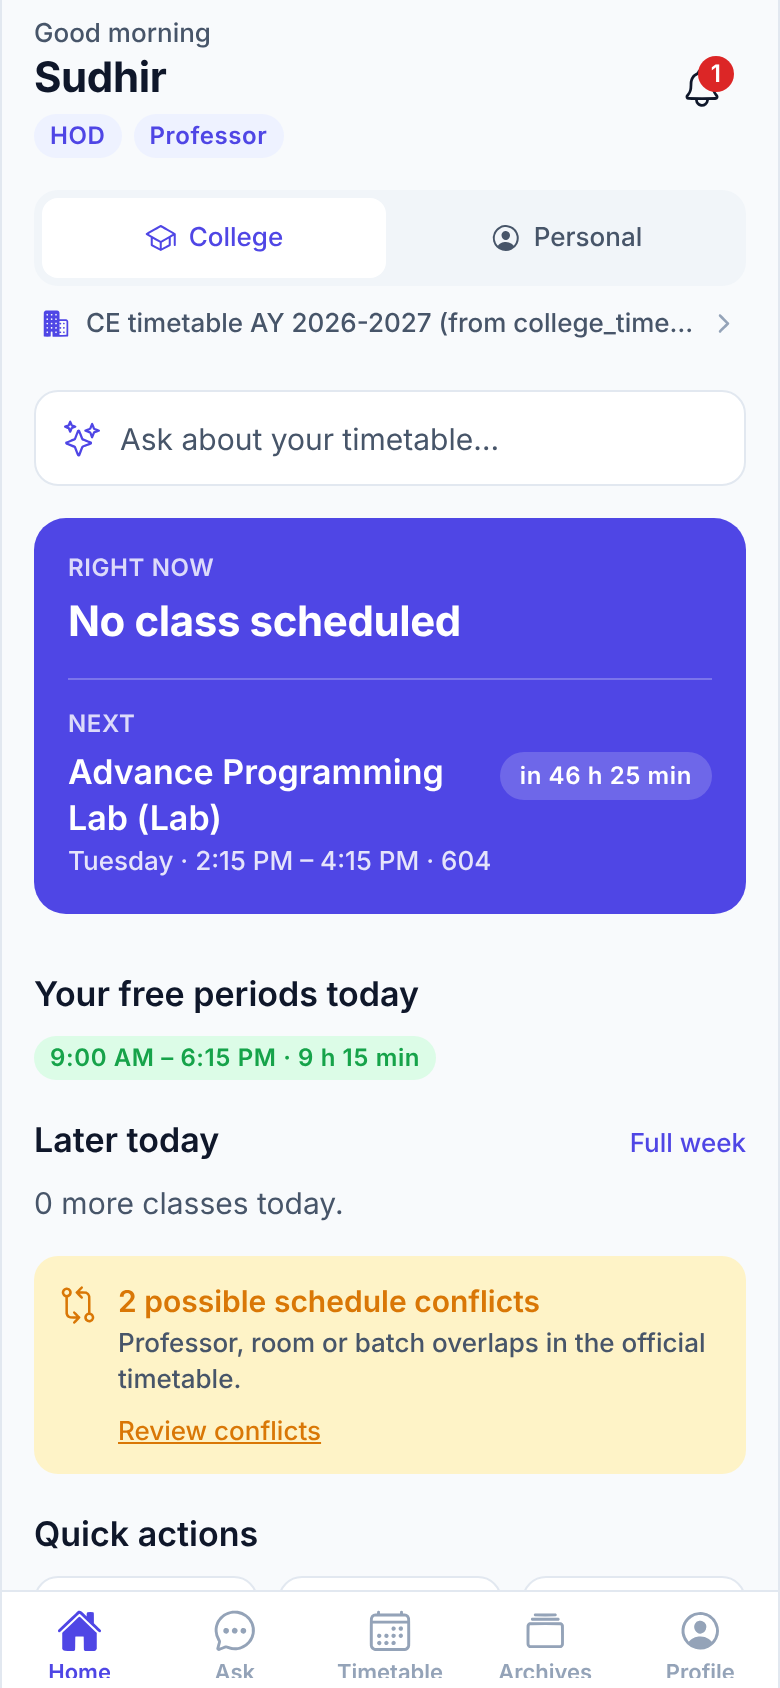
\includegraphics[width=\linewidth]{figures/screens/hod-home.png}\caption{HOD home with conflict alert}\end{subfigure}\hfill
\begin{subfigure}[t]{0.24\textwidth}\centering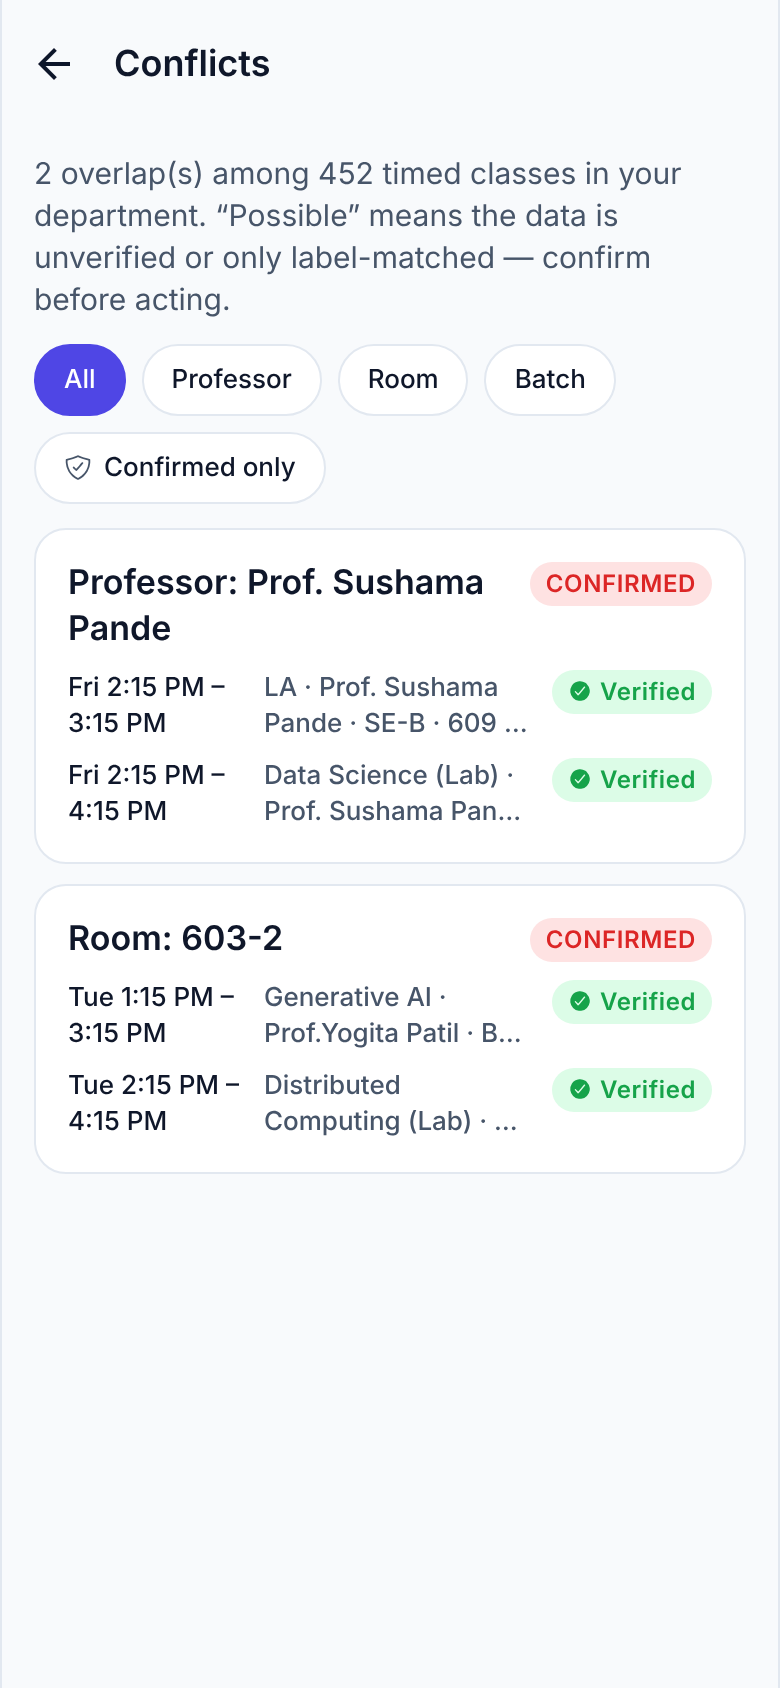
\includegraphics[width=\linewidth]{figures/screens/conflicts.png}\caption{The 2 genuine clashes}\end{subfigure}\hfill
\begin{subfigure}[t]{0.24\textwidth}\centering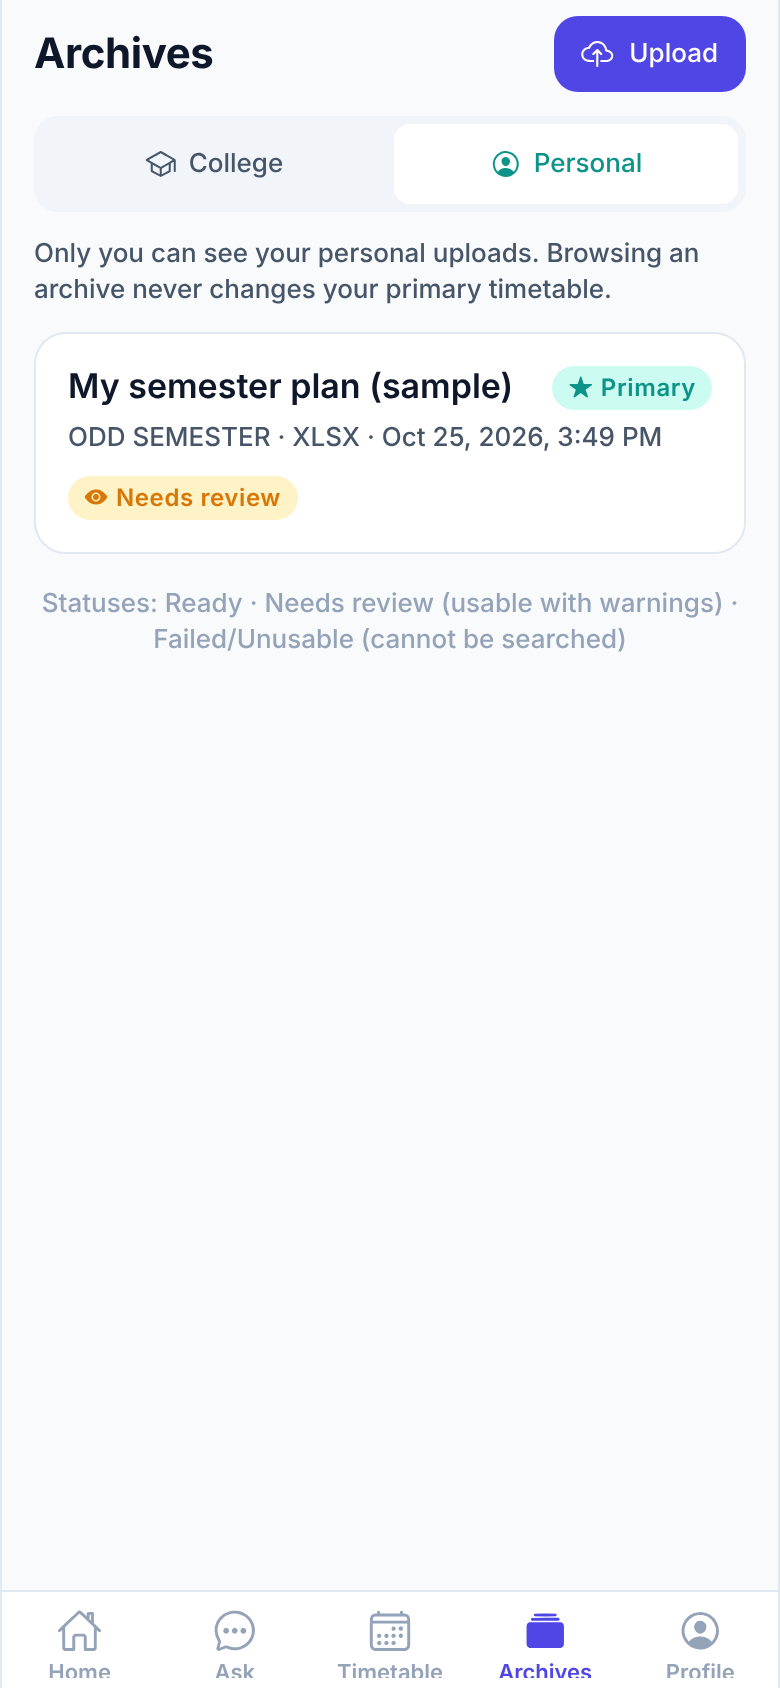
\includegraphics[width=\linewidth]{figures/screens/personal-archives.png}\caption{Personal archives (private)}\end{subfigure}
\caption{Combined classes, HOD view, conflicts and personal domain}
\label{fig:screens2}
\end{figure}

\begin{figure}[H]
\centering
\begin{subfigure}[t]{0.24\textwidth}\centering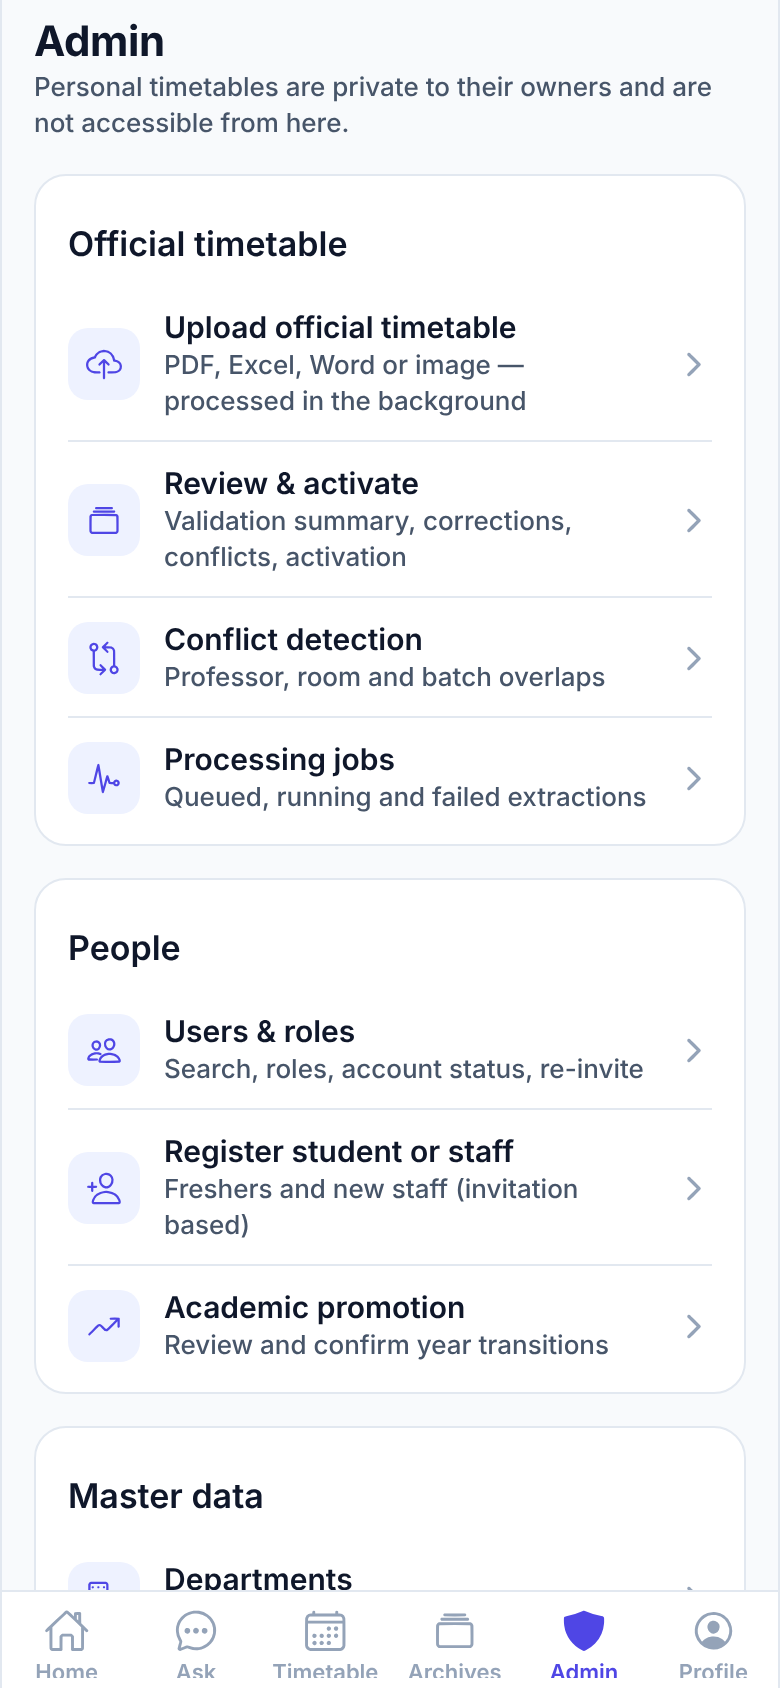
\includegraphics[width=\linewidth]{figures/screens/admin-hub.png}\caption{Admin hub}\end{subfigure}\hfill
\begin{subfigure}[t]{0.24\textwidth}\centering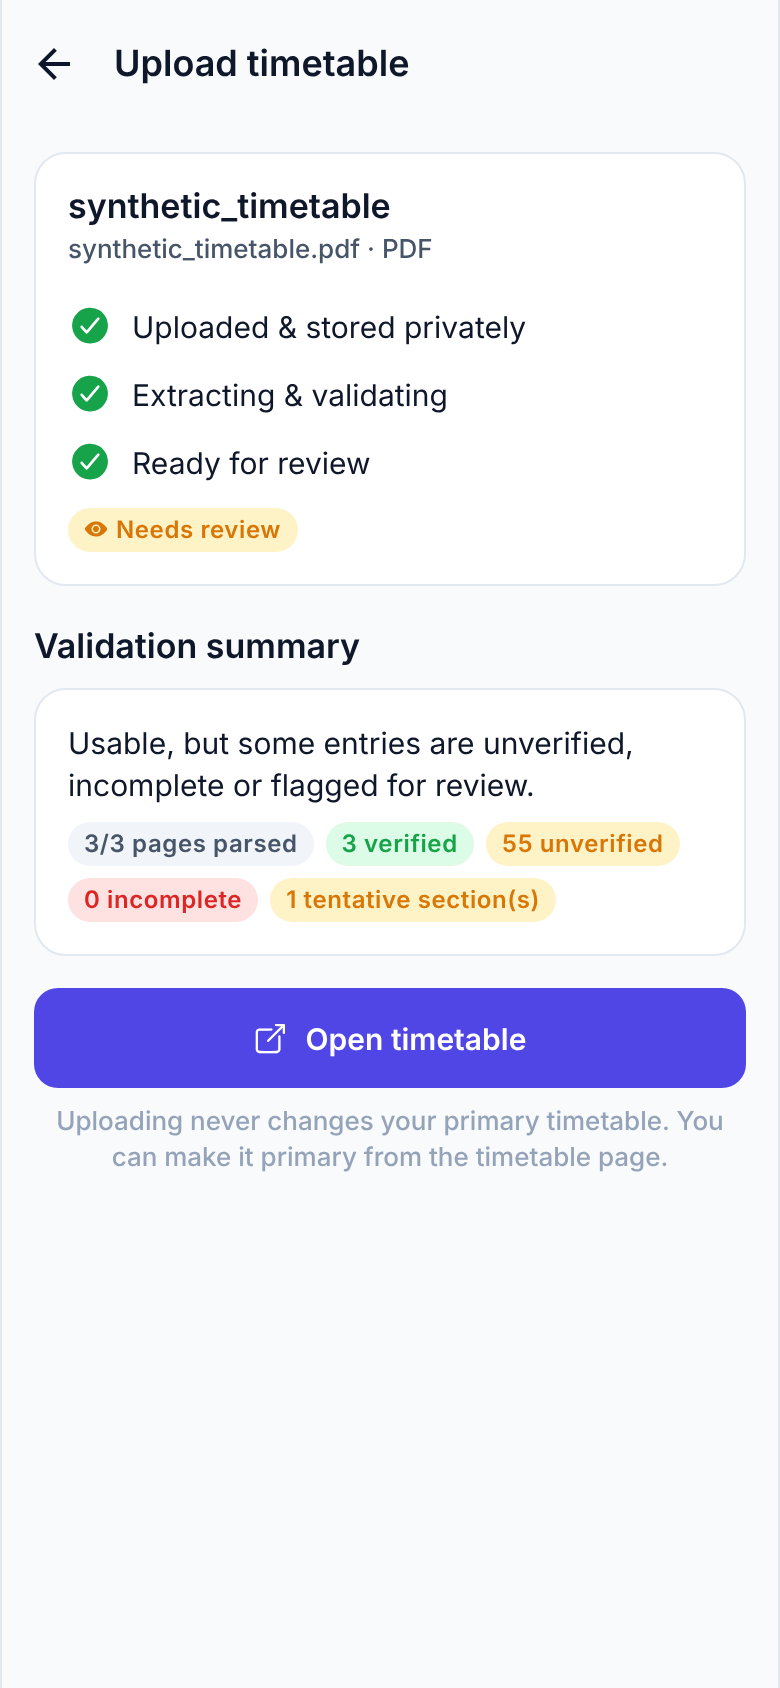
\includegraphics[width=\linewidth]{figures/screens/upload-processed.png}\caption{Upload processed by worker}\end{subfigure}\hfill
\begin{subfigure}[t]{0.24\textwidth}\centering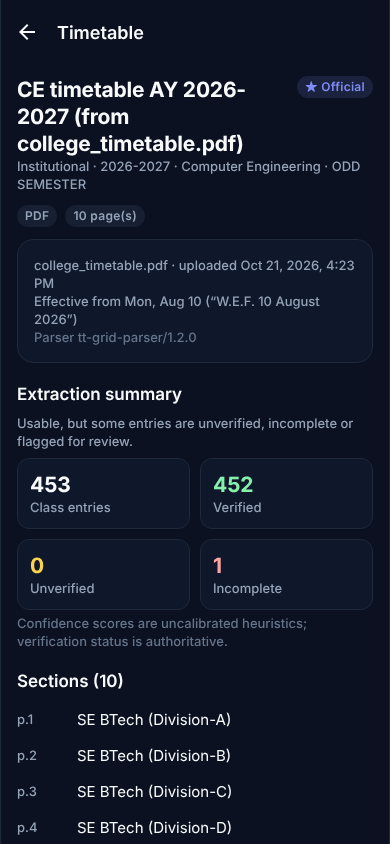
\includegraphics[width=\linewidth]{figures/screens/real-timetable-summary.png}\caption{Real PDF: 453 entries, 452 verified, 10 sections}\end{subfigure}
\caption{Administrator workflow}
\label{fig:screensadmin}
\end{figure}

\begin{figure}[H]
\centering
\begin{subfigure}[t]{0.31\textwidth}\centering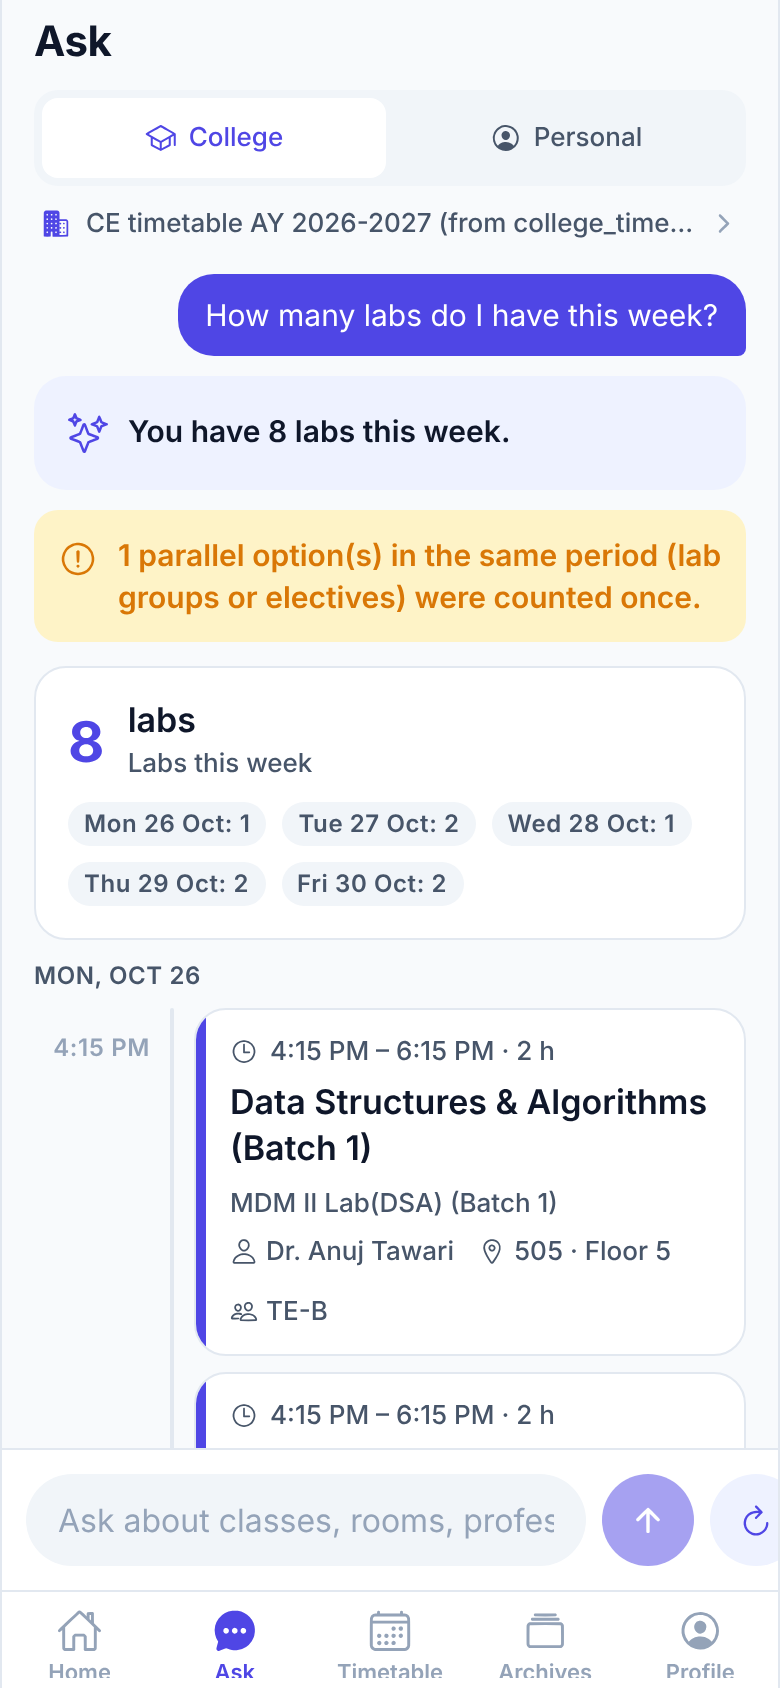
\includegraphics[width=\linewidth]{figures/screens/composed-count.png}\caption{``How many labs do I have this week?'': count with per-day breakdown}\end{subfigure}\hfill
\begin{subfigure}[t]{0.31\textwidth}\centering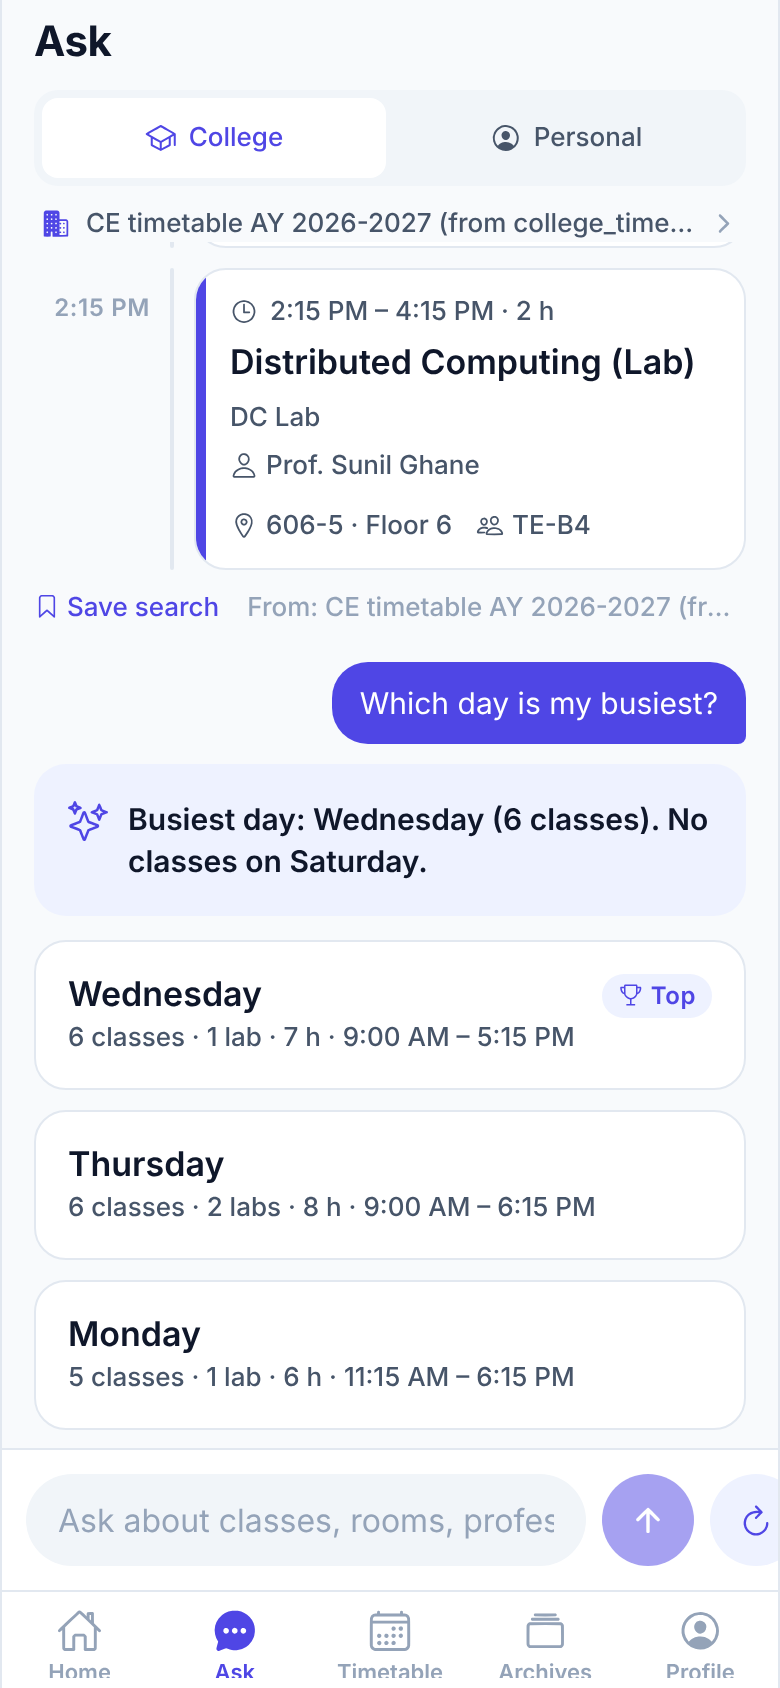
\includegraphics[width=\linewidth]{figures/screens/composed-busiest.png}\caption{``Which day is my busiest?'': day-wise summary}\end{subfigure}\hfill
\begin{subfigure}[t]{0.31\textwidth}\centering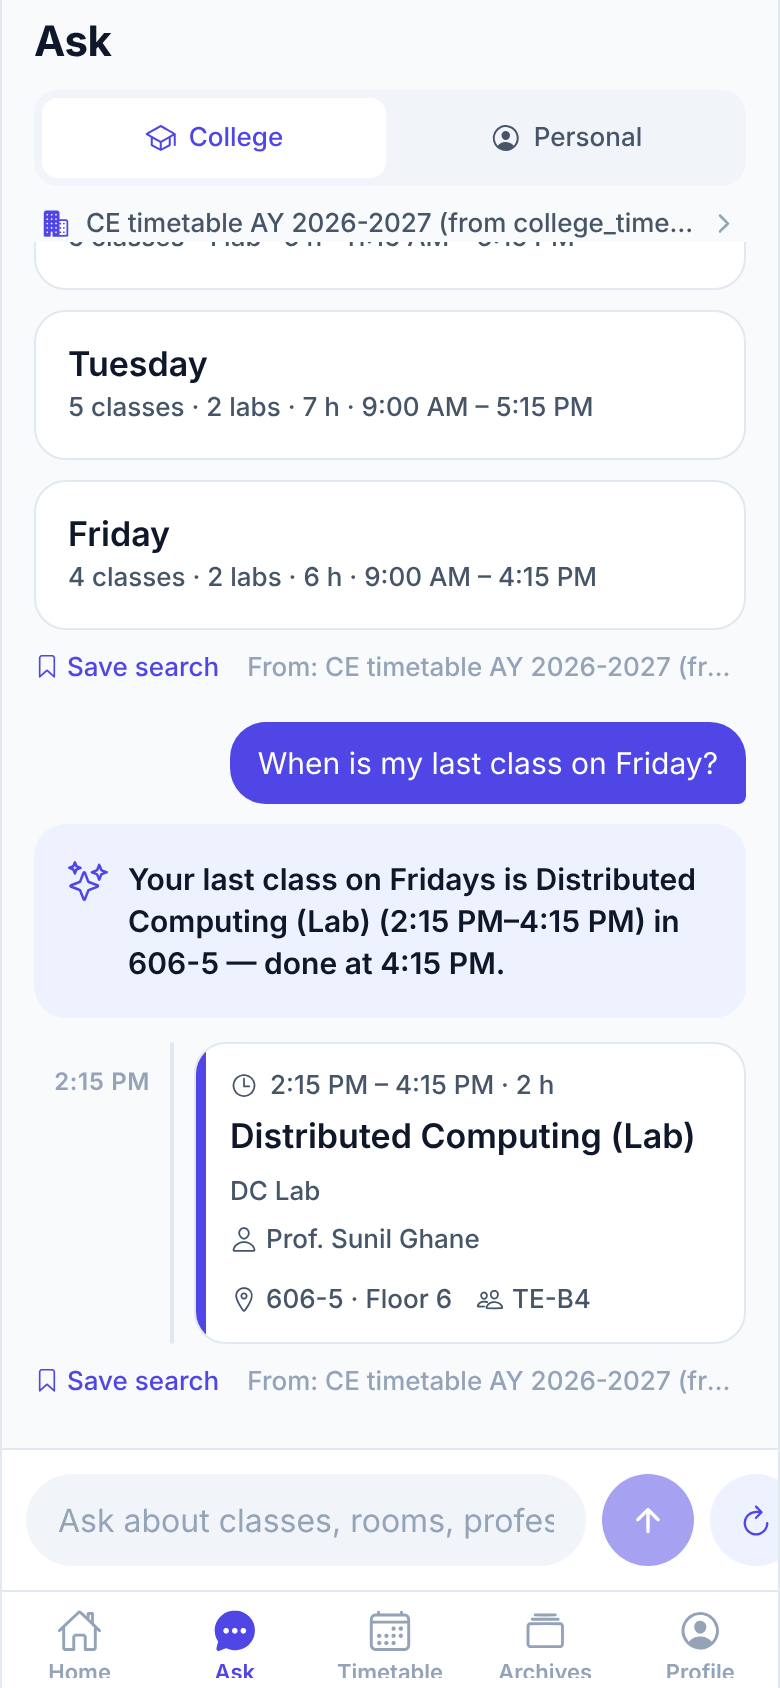
\includegraphics[width=\linewidth]{figures/screens/composed-last.png}\caption{``When is my last class on Friday?''}\end{subfigure}
\caption{Composed query plans answered from the real timetable (TE-B4 student)}
\label{fig:screenscomposed}
\end{figure}

\begin{figure}[H]
\centering
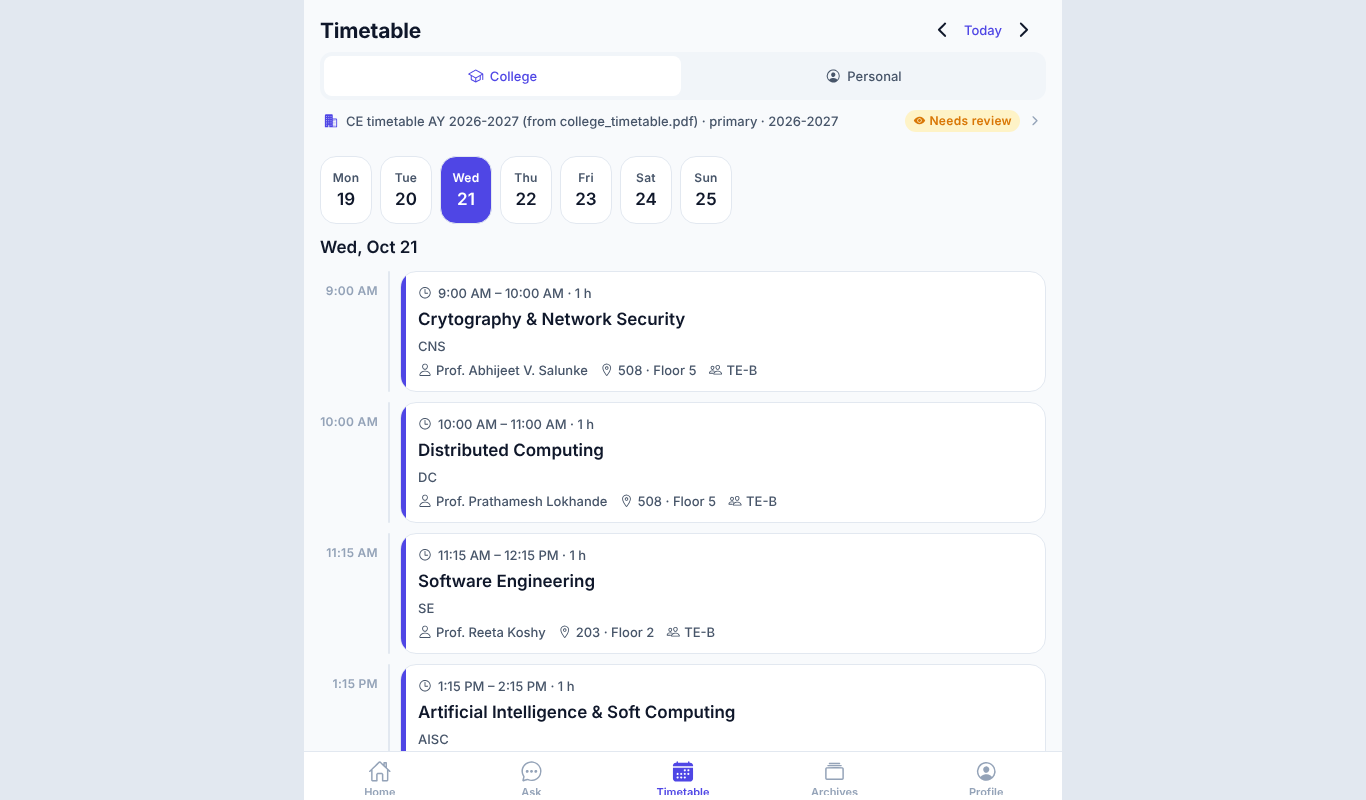
\includegraphics[width=0.8\textwidth]{figures/screens/laptop-timetable.png}
\caption{The same app in a laptop browser}
\label{fig:laptop}
\end{figure}

\subsection{Functional Results}
\begin{itemize}
\item \textbf{Extraction (FR-04):} the real PDF (10 pages, 420~kB) produced 570 rows: 453 class entries,
      of which \textbf{452 verified} and 1 \textsc{Incomplete} (M.Tech.\ HSS on Friday has no time
      label in the PDF), plus breaks and activities. All 10 pages were parsed, and 46 batches, 38
      courses, 52 faculty and 42 rooms were recognised.
\item \textbf{Conflicts (FR-13):} exactly two clashes, both confirmed by hand in the PDF:
      (1) \emph{Friday 2:15--3:15}, Prof.\ Sushama Pande has \emph{LA} for SE-B in 609 (page 2) and
      \emph{Data Science Lab C3} for SE-C in 606-4 (page 3); (2) \emph{Tuesday 2:15--3:15}, room
      \textbf{603-2} has B.E.\ \emph{PE III -- Gen AI} (page 9) and TE-D \emph{DC Lab D2} (page 8).
\item \textbf{Role views (FR-09/10):} SE-A1 sees only A1's labs on Wednesday; B.E.\ A and C both see
      the combined B.E.\ electives; LLC appears without teacher or room; the noon row 12:15--13:15 is a
      normal class.
\item \textbf{Queries (FR-11):} ``Do I have classes after lunch?'' uses 14:15 for S.E.\ and 13:15
      for T.E.\ (each from its own section). ``Am I free at 2?'' asks a.m./p.m. A student without a
      batch gets a setup message instead of an invented answer.
\item \textbf{Privacy (FR-14):} another user's personal timetable returns 404, even for the Admin.
\end{itemize}

\subsection{Performance Results}
Summarised from Chapter~8: median search latency 37--47~ms for a single user; 46.5~req/s at 4
clients and about 55--60~req/s at saturation with 4 workers on a 4-core VM; 0 wrong answers in 960
requests at 32 clients; extraction of the 10-page PDF in 1.65~s using 82~MB peak memory; 12~MB
database.

\begin{figure}[H]
\centering
\begin{tikzpicture}
\begin{axis}[ybar,width=0.9\textwidth,height=5.2cm,bar width=16pt,ymin=0,ymax=680,
  symbolic x coords={Naive overlaps,After rule set 1,After rule set 2},xtick=data,
  nodes near coords,ylabel={Reported conflicts},enlarge x limits=0.25,title={\small Conflict reports on the real PDF}]
\addplot[fill=spitblue!60] coordinates {(Naive overlaps,542) (After rule set 1,25) (After rule set 2,2)};
\end{axis}
\end{tikzpicture}
\caption{Effect of intended-overlap rules: from 542 raw overlaps to the 2 genuine clashes}
\label{fig:conflictbar}
\end{figure}

\subsection{Comparison with Existing Systems}
Using the criteria of Table~\ref{tab:compare}, the proposed system is the only one that reads the
published timetable and also answers role-scoped questions safely. Table~\ref{tab:effort} compares
the effort for common tasks. The manual times are our own estimates from trying each task with the PDF;
they were not measured in a controlled study.

\begin{table}[H]
\centering
\caption{Task effort: manual PDF lookup vs.\ the app (manual times are estimates)}
\label{tab:effort}
\small
\begin{tabularx}{\textwidth}{@{}Xp{3.5cm}p{3.5cm}@{}}
\toprule
\textbf{Task} & \textbf{Manual PDF} & \textbf{Dynamic Timetable}\\
\midrule
Find my next class and its room & find page, row, column, lab group, legend: about 1 min & open app: 0 taps\\
Find a free room at 11~am on floor 6 & check every page for every room: 10+ min & one question, $<$1 s\\
Check all teacher/room clashes & impractical by hand (453 classes) & automatic, on every upload\\
Know whether the timetable changed & compare two PDFs by eye & notification + archive\\
Lab-group view (A1 vs A2) & read the stacked cells carefully & filtered automatically\\
\bottomrule
\end{tabularx}
\end{table}

\subsection{Achievement of Objectives}
\begin{table}[H]
\centering
\caption{Objectives mapped to evidence}
\label{tab:objectives}
\small
\begin{tabularx}{\textwidth}{@{}p{0.8cm}Xp{1.9cm}@{}}
\toprule
\textbf{Obj.} & \textbf{Evidence} & \textbf{Status}\\
\midrule
O1 & 99.8\% verified on the real PDF; uncertain values flagged (TC-07, TC-09) & Achieved\\
O2 & PDF, scanned PDF/photo (OCR), XLSX/XLS, CSV, DOCX/DOC through one pipeline (TC-04, TC-10) & Achieved\\
O3 & Five roles, server-side policy, role tests (TC-03), dashboards (Fig.~\ref{fig:screens1}, \ref{fig:screens2}) & Achieved\\
O4 & Specialised operations plus composed query plans (counts, first/last, day-wise, lab/lecture), with clarification (TC-16--TC-19, TC-31--TC-34) & Achieved\\
O5 & 2 genuine clashes, 0 false reports (TC-21) & Achieved\\
O6 & Separate tables; IDOR and isolation tests (TC-22); archives & Achieved\\
O7 & p50 37--47 ms; 0 wrong answers at 32 clients (TC-28, TC-29) & Achieved (dev hardware)\\
O8 & Android/iPhone via Expo Go, laptop browser, Render demo & Achieved; store builds pending\\
O9 & 168 + 20 + 45 e2e steps passing & Achieved\\
\bottomrule
\end{tabularx}
\end{table}

\subsection{Discussion of Findings}
\begin{itemize}
\item \textbf{Real data is different from specifications.} Most of the extraction work went into
      conventions found only in the real PDF: the mislabelled noon row, codes missing from legends, LLC
      slots and combined B.E.\ pages. Testing on the real document from early on was decisive.
\item \textbf{Honest uncertainty builds trust.} Marking the one entry without a time as
      \textsc{Incomplete}, instead of guessing, kept every automatic answer correct.
\item \textbf{The source document itself had errors.} The two clashes are real errors in the
      published timetable, so the system already adds value for the timetable committee.
\item \textbf{Unexpected observation:} a small connectivity check (\texttt{HEAD /}) made the whole
      production web app appear offline. This shows why end-to-end tests in a production-like
      configuration matter.
\item \textbf{Rules beat a black box here, if they compose.} A fixed list of question types felt limiting
      (counts, ``busiest day'', ``last lab on Friday'' were refused). Making the rules compose into a query
      plan removed most of that limit while keeping reproducible answers in about 40~ms, no API cost and
      no injection risk.
\end{itemize}

\subsection{Practical Applicability}
The department can use the system as it is for the current semester: the Admin uploads the
official PDF, reviews the flagged entry, activates it, and students and faculty use the web link
or the app. Before full-college use, the college should provide always-on hosting, e-mail for account
activation, and store builds of the app (Section~11.5). The approach also transfers to other
departments and institutes that publish grid-style timetables. Their layouts may need parser
adjustments, which the review workflow and regression tests are designed for.

\newpage
